\documentclass[10pt,a4paper]{article}
\usepackage[T1]{fontenc}
\usepackage{amssymb}
\usepackage[left=2.25cm,right=2.25cm,top=2.25cm,bottom=2.75cm]{geometry}
\usepackage{graphicx}
\usepackage{isabelle}
\usepackage{isabellesym}
\usepackage[only,bigsqcap]{stmaryrd}
\usepackage{pdfsetup}

\urlstyle{tt}
\isabellestyle{it}

% for uniform font size
%\renewcommand{\isastyle}{\isastyleminor}

\renewcommand{\isacharunderscore}{\_}

\begin{document}

\title{A Verified Functional Implementation of \\ Bachmair and Ganzinger's Ordered Resolution Prover}
\author{Anders Schlichtkrull, Jasmin Christian Blanchette, and Dmitriy Traytel}

\maketitle

\begin{abstract}
\noindent
This Isabelle/HOL formalization refines the abstract ordered resolution prover
presented in Section~4.3 of Bachmair and Ganzinger's ``Resolution Theorem
Proving'' chapter in the \emph{Handbook of Automated Reasoning}. The result
is a functional implementation of a first-order prover.
\end{abstract}

\tableofcontents

% sane default for proof documents
\parindent 0pt
\parskip 0.5ex

\section{Introduction}

Bachmair and Ganzinger's ``Resolution Theorem Proving'' chapter
%\cite{bachmair-ganzinger-2001}
in the \emph{Handbook of Automated Reasoning} is the standard reference on the
topic. It defines a general framework for propositional and first-order
resolution-based theorem proving. Resolution forms the basis for
superposition, the calculus implemented in many popular automatic theorem
provers.

\medskip

This Isabelle/HOL formalization starts from an existing formalization of
Bachmair and Ganzinger's chapter, up to and including Section 4.3. It refines
the abstract ordered resolution prover presented in Section~4.3 to obtain an
executable, functional implementation of a first-order prover.
Figure~\ref{fig:thys} shows the corresponding Isabelle theory structure.

\medskip

We refer to the following conference paper for details:

\begin{quote}
Anders Schlichtkrull, Jasmin Christian Blanchette, Dmitriy Traytel: \\
A verified prover based on ordered resolution. \\
CPP 2019: 152-165 \\
\url{http://matryoshka.gforge.inria.fr/pubs/fun_rp_paper.pdf}
\end{quote}

\begin{figure}
\begin{center}
  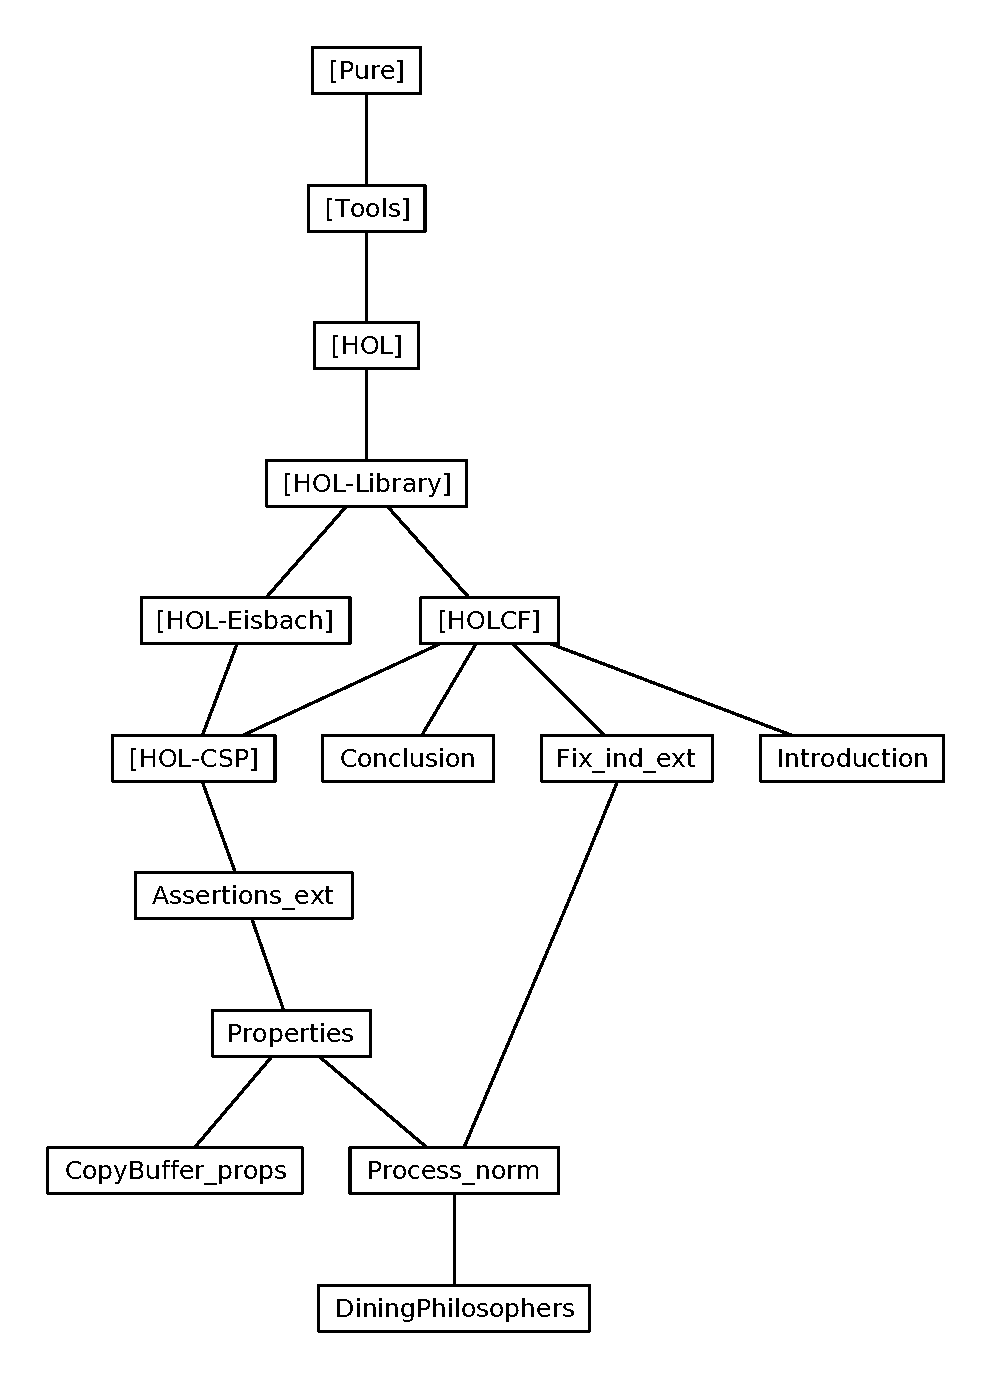
\includegraphics[width=0.75\textwidth,keepaspectratio]{session_graph}
\end{center}
\caption{Theory dependency graph}
\label{fig:thys}
\end{figure}

% generated text of all theories
\input{session}

% optional bibliography
% \bibliographystyle{abbrv}
% \bibliography{bib}

\end{document}
